\section{Autonomous Vehicle}
\label{sec:bicycle}

\subsection{Example Description}
This pilot study is an example of a vehicle driving a route defined from a set of way points. The multi-model consist of a steering controller and a model representing the dynamics of a vehicle. The steering controller contains the desired route of the vehicle. The vehicle is steered on the front wheels. 

\begin{figure}[htbp]
\begin{center}
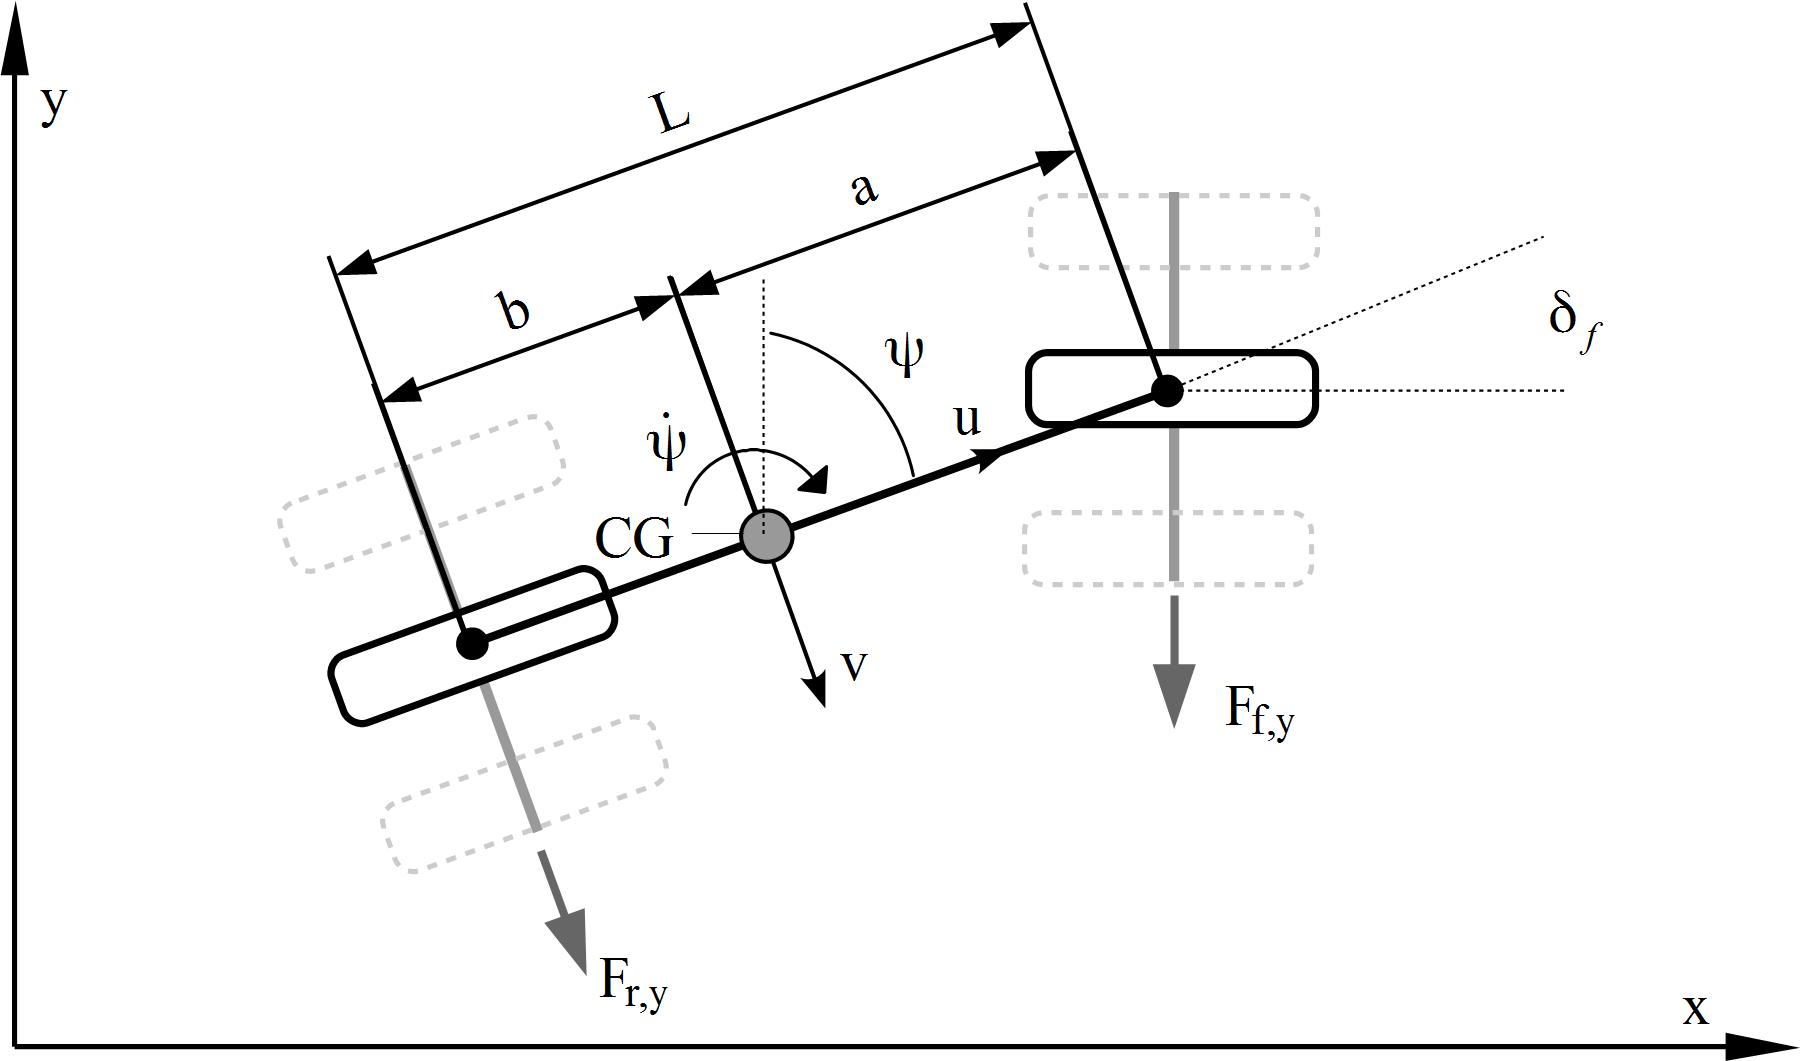
\includegraphics[width=0.6\textwidth]{vehicle/bicycle.png}
\caption{Overview and notation of the vehicle}
\label{fig:bicyclemodel_overview}
\end{center}
\end{figure}

\subsection{Usage} \label{sec:bicycle_usage}
The autonomous vehicle pilot study is an example of a vehicle driving through a path of specified way points. The example is available on \texttt{https://github.com/into-cps/case-study\_vehicle}. 

The folder \texttt{FMUs} contains \texttt{vehicle.fmu} and \texttt{steering\_controller.fmu}. The folder \texttt{Models} contains the VDM-RT project of the steering controller and the 20sim model of the dynamic description of the vehicle, \texttt{BicycleModel.emx}. The folder \texttt{Multi-models} contains the multi-model definition.  

To run a simulation, open the INTO-CPS application, expand the \texttt{basic-sim} folder and open \texttt{Simulation-1}. Launch the COE and hit `Simulate'. 
By default, the simulation integrates with a fixed time step size of 0.1 second for 100 seconds. \newline

After a finished simulation, visualize the trajectory by running the file, \texttt{plot\_trajectory.py} that illustrates the trajectory of the latest simulation in the folder \texttt{\textbackslash Multi-models\textbackslash si\-mu\-la\-tion-1}. 

\subsection{INTO-CPS SysML profile}
The autonomous vehicle study SysML model is constructed using the the INTO-CPS profile. The Architecture Diagram of the co-simulation is shown in Figure~\ref{fig:bicycle_architecture_diagram},the Connection Diagram is shown in Figure~\ref{fig:bicycle_connection_diagram}.
In the \textit{RouteFollowingSystem} contains the \textit{vehicle} component and component \textit{Controller}. Position and orientation of the vehicle is passed between the two components. From \textit{Vechicle} the current position is passed to the controller in where the desired orientation is determined based on the route and converted to a steering angle \texttt{delta\_f}. 
	\begin{figure}[htbp]
	\begin{center}
		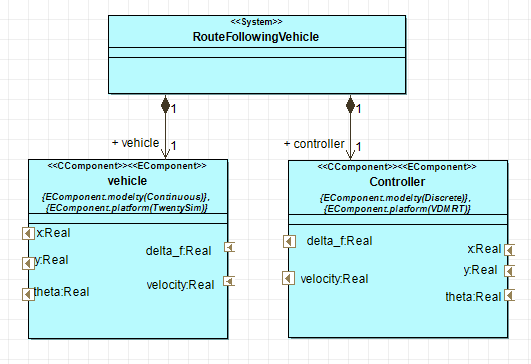
\includegraphics[width=0.6\textwidth]{vehicle/architecture_structure_diagram.png}
		\caption{Architecture Diagram}
		\label{fig:bicycle_architecture_diagram}
	\end{center}
\end{figure}
\begin{figure}[htbp]
	\begin{center}
		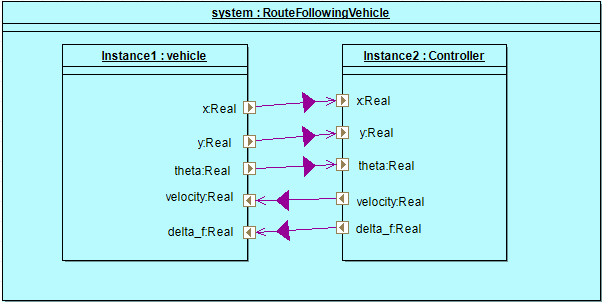
\includegraphics[width=0.6\textwidth]{vehicle/connection_diagram.png}
		\caption{Connection Diagram}
		\label{fig:bicycle_connection_diagram}
	\end{center}
\end{figure}

\subsection{Multi-model}
\label{sec:bicycle_mm}
The parameters of the simulation can be changed in the INTO-CPS application or through the \texttt{mm.json} file.  
\subsubsection{Models}
\label{sec:bicycle_models}
The SysML model above shows that the multi-model consists of two separate models. A 20sim model of the dynamic behaviour of the vehicle and a steering controller that keeps the vehicle on the specified path. 

\begin{description}
	\item[BicycleModel.emx] The 20-sim model of the \emph{vehicle} component, shown in Figure~\ref{fig:vehicle_20sim}, contains several components. 	
	\begin{figure}[htbp]
		\begin{center}
			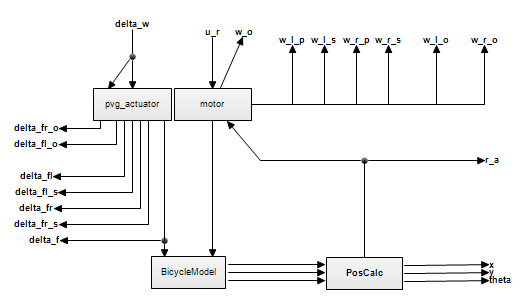
\includegraphics[width=0.8\textwidth]{vehicle/vehicle.png}
			\caption{20-sim vehicle model}
			\label{fig:vehicle_20sim}
		\end{center}
	\end{figure}

The actuation block, \texttt{pvg\_actuator} converts the desired steering angle from the controller to an steering angle compliant with the mechanical system. The actuation is shown in Figure~\ref{fig:pvg_actuation_20sim}. \texttt{delta\_fl\_w} and \texttt{delta\_fr\_w} are the desired steering angles. \texttt{delta\_f} is the angle applied in the vehicle dynamics calculations. \texttt{delta\_f} is calculated as the average of the two angle components from left and right side.   
	\begin{figure}[htbp]
		\begin{center}
			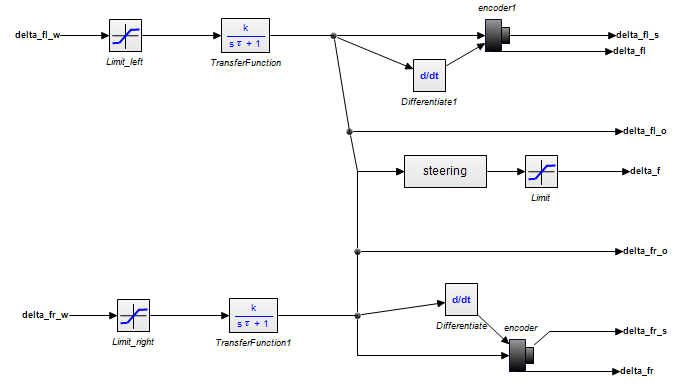
\includegraphics[width=0.8\textwidth]{vehicle/Steering_actuator.png}
			\caption{Actuation system}
			\label{fig:pvg_actuation_20sim}
		\end{center}
	\end{figure}
	
	The \texttt{BicycleModel} components holds the calculations of the dynamic bicycle model. The \texttt{BicycleModel} is shown in Figure~\ref{fig:bicyclemodel_20sim}. The inputs to the model are the the forward velocity of the vehicle \texttt{u\_r} and the \texttt{delta\_f} which is the steering angle as shown in Figure~\ref{fig:bicyclemodel_overview}. The outputs are the velocity components in $x$ and $y$ direction and yaw-rate \texttt{d\_x\_v}, \texttt{d\_y\_v} and \texttt{r}.  
	\begin{figure}[htbp]
	\begin{center}
		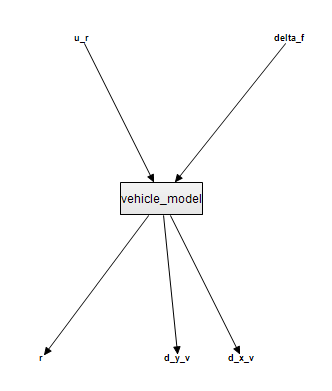
\includegraphics[width=0.4\textwidth]{vehicle/Bycycle_model.png}
		\caption{BicycleModel}
		\label{fig:bicyclemodel_20sim}
	\end{center}
	\end{figure}
	
	The \texttt{vehicle\_model} contains the following initial equations determining the weight on the wheels, the position of the centre of gravity (CG) and the moment of inertia as shown in Figure~\ref{fig:initial_equations}. 
	\begin{figure}[htbp]
	\begin{center}
		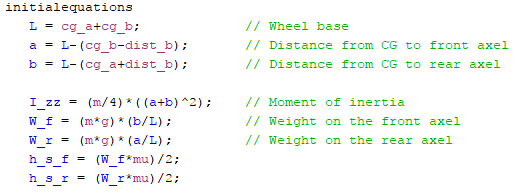
\includegraphics[scale=1]{vehicle/initial_equations.png}
			\caption{\texttt{initialequations}}
			\label{fig:initial_equations}
	\end{center}
	\end{figure}
	An important feature of vehicle dynamics is the estimation of the lateral tire forces. These are in this case calculated with a non-linear tire model. The calculation of the slipangles and the lateral tire forces is determined as shown in Figure~\ref{fig:tire_model}.
		\begin{figure}[htbp]
		\begin{center}
			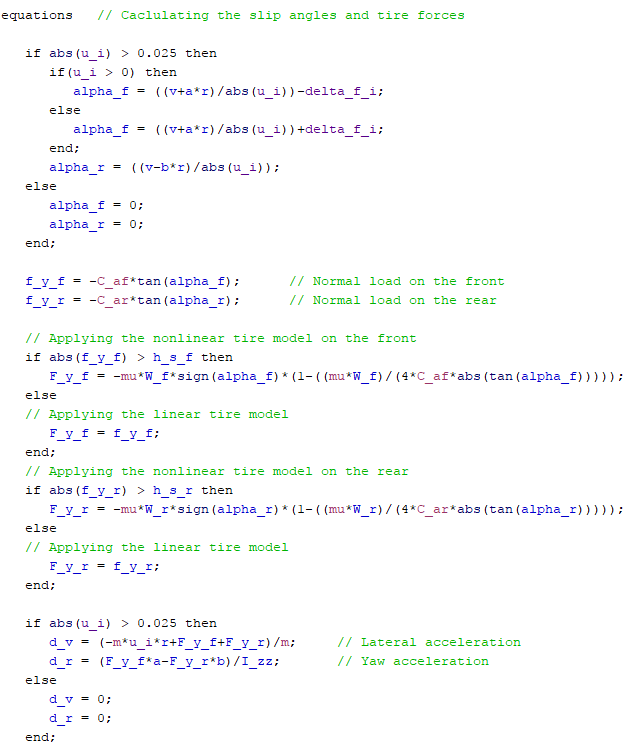
\includegraphics[width = 1\linewidth]{vehicle/tire_model.png}
			\caption{\texttt{Tire model}}
			\label{fig:tire_model}
		\end{center}
	\end{figure}


	\item[steering\_controller] is a VDM-RT project. The \textit{System} class contains a \textit{HardwareInterface} with RealPorts where the position and orientation of the vehicle is passed into the control calculations. 
	The control signal is calculated as the product of a gain (p) and the angular misalignment of the current heading of the vehicle and the desired heading towards the next way point. 
	An illustration of the steering controller is shown in \ref{fig:controller} where $x$ and $y$ is the current position.
	\begin{figure}[htbp]
		\begin{center}
			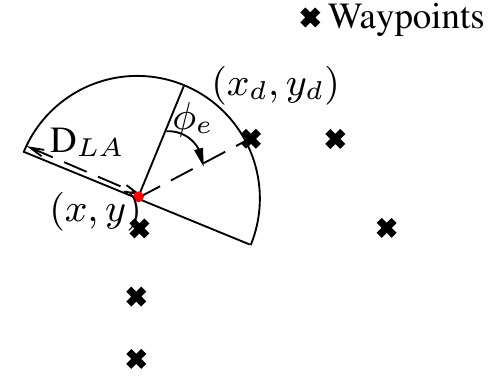
\includegraphics[width = 0.4\linewidth]{vehicle/controller_sketch.png}
			\caption{Sketch of steering control, $ \left(x,y\right) $ is the current position of the lawn mower, $ \left(x_d,y_d\right)$ is the desired heading, and $\phi_e$ is the deviation.}
			\label{fig:controller}
		\end{center}
	\end{figure}
	The route is specified in a \texttt{.csv} file in the folder \texttt{...\textbackslash Models\textbackslash steering\_controller}.
\end{description}




\subsubsection{Configuration}
\label{sec:bicyclemodel_conf}
One multi-models is defined: The model corresponds to the connection diagram shown in Figure~\ref{fig:bicycle_architecture_diagram}. 


\subsection{Co-simulation}
A co-simulation is performed through the INTO-CPS application for 180 seconds using a fixed time-step of 0.1 sec. 
The parameters of simulation is defined in the mm.json as : \\
\texttt{"\{fmu1\}.Steering\_control.speed\_ref": 1,} \\
\texttt{"\{fmu1\}.Steering\_control.look\_ahead\_dist": 1,} \\
\texttt{"\{fmu1\}.Steering\_control.control\_parameter": 1}. \\

Running the simulation in the INTO-CPS application, the results are presented in Figure~\ref{fig:results1}. The graphs \texttt{vehicle.x} and \texttt{vehicle.y} represents the relative position in meters compared to the initial point of the vehicle. \texttt{Steering\_control.speed} is the forward velocity of the vehicle in m/s and \texttt{Stee\-ring\_con\-trol.delta\_f} is the steering angle in radians. 

\begin{figure}[!h]
	\begin{center}
		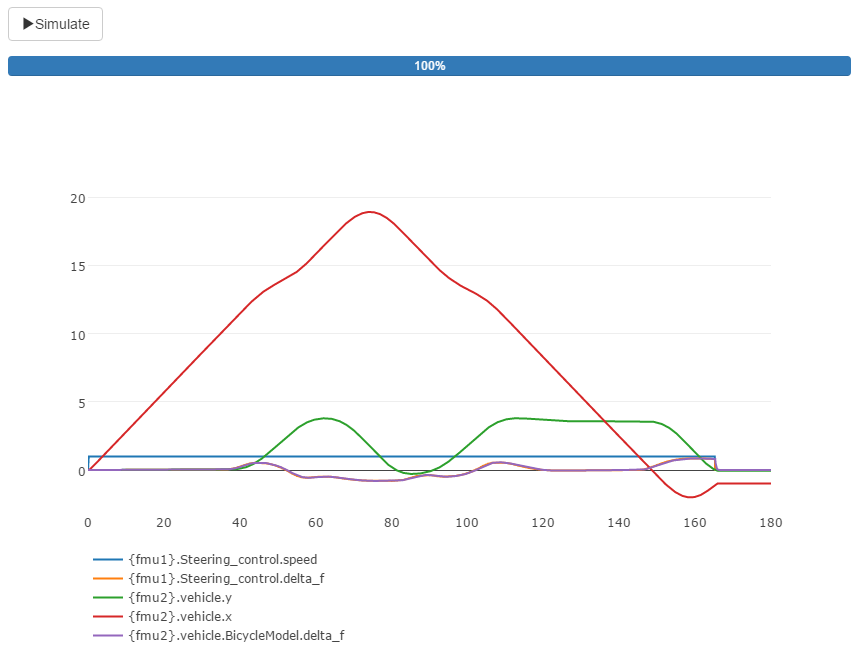
\includegraphics[width=0.8\textwidth]{vehicle/result1.png}
		\caption{Simulation results in the the INTO-CPS app}
		\label{fig:results1}
	\end{center}
\end{figure}

By plotting the x and y components, the trajectory reveals, as shown in Figure~\ref{fig:results1a}. The blue dashed line is the desired route, and the red graph is the simulated trajectory.

\begin{figure}[!h]
	\begin{center}
		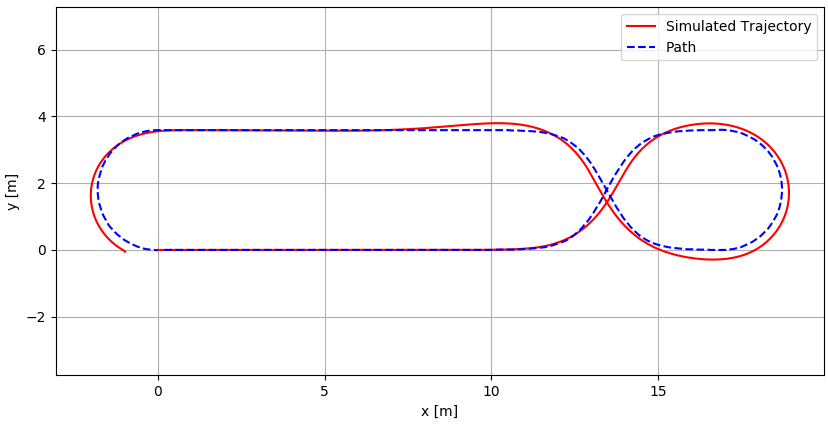
\includegraphics[width=0.6\textwidth]{vehicle/result1a.png}
		\caption{Simulation results in the the INTO-CPS application}
		\label{fig:results1a}
	\end{center}
\end{figure}
\subsection{Analyses and Experiments}
The performance, e.g. how well the vehicle track the desired route, can be investigated by changing the parameters in the \texttt{mm} file. Hereby, the influence of the control parameter p and the look ahead distance of the controller be evaluated under different velocities.  
\subsubsection{Design Space Exploration}
The DSE features are available for this pilot study. An objective script has been reused from the Line-following Robot pilot study, the \textit{meanCrosstrackError}. For further information, see Section \ref{sec:linefollwerrobot}. 
In this example, a simple DSE is presented. The DSE evaluates the mean cross track error as a function of the velocity, gain and look-ahead parameter. In this example, an exhaustive search is applied for exploiting the design space in a number of predefined values.
The parameters applied here is defined in the dse.json file as follows:\\
\texttt{"\{fmu1\}.Steering\_control.speed\_ref":  [0.5, 1.0]} \\
\texttt{"\{fmu1\}.Steering\_control.look\_ahead\_dist": [0.5, 1.0]} \\
\texttt{"\{fmu1\}.Steering\_control.control\_parameter": [0.5, 1.0]}, \\
giving a total of $2^3=8$ simulations. The results are ranked only based on the mean cross track error as shown in Figure~\ref{fig:ranking} from the \texttt{results.html} file.  
The column \texttt{mean\-Cross\-Track\-Error2} is forced to \texttt{1.0} since the designs has only been evaluated based on the mean cross track error. This is forces through the file \texttt{one\_function.py} in the userMetricScripts folder. 

\begin{figure}[htbp]
	\begin{center}
		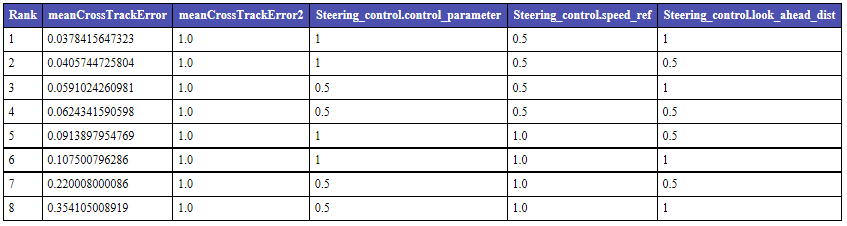
\includegraphics[width=1\textwidth]{vehicle/rank.png}
		\caption{Ranking}
		\label{fig:ranking}
	\end{center}
\end{figure}
Which illustrates that the best combination of parameters in terms of tracking the route is the combination of look-ahead and control parameter p is [1.0, 1.0] at a velocity of 0.5 m/s.